\documentclass{homeworg}
\usepackage{amsmath}

\title{Travail 2 - Circuits DC - Méthode des noeuds}
\author{Wats Raphaël}

\begin{document}
\maketitle

\section{Schéma du circuit}
    \begin{center}
        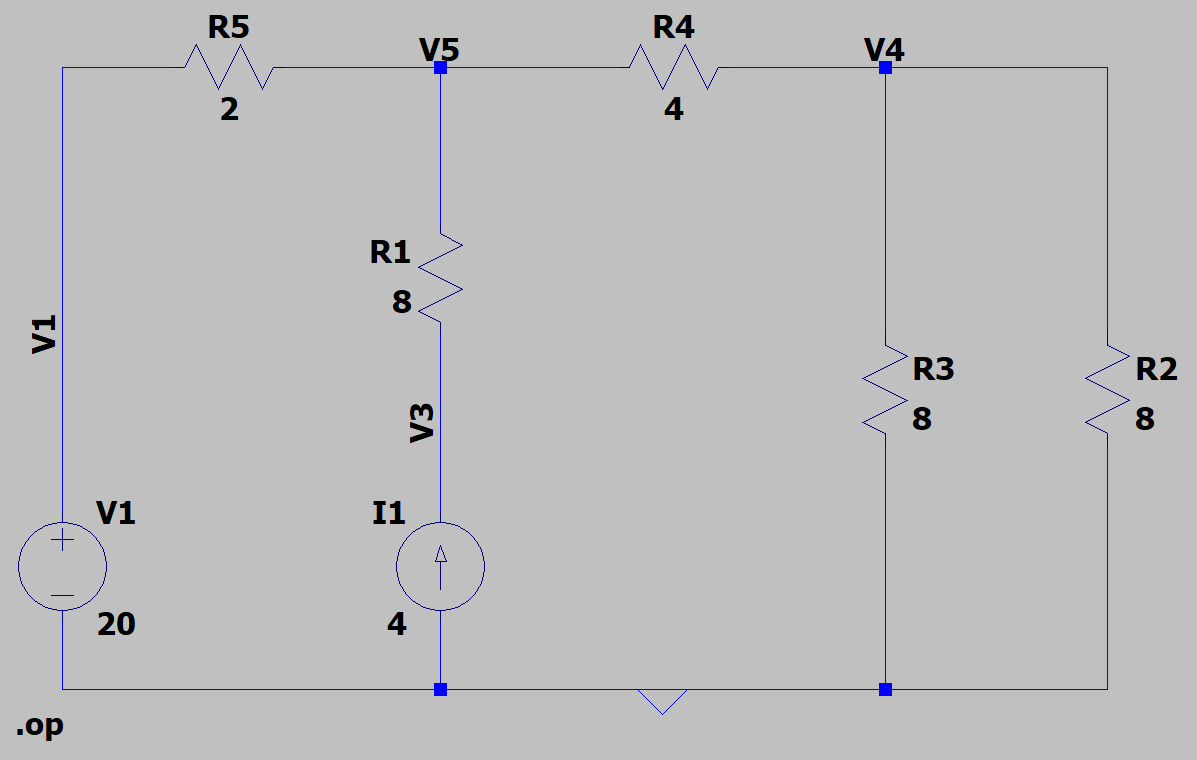
\includegraphics[scale=0.5]{Shematic.PNG}
    \end{center}

\section{Détail des calculs}
    \begin{center}
        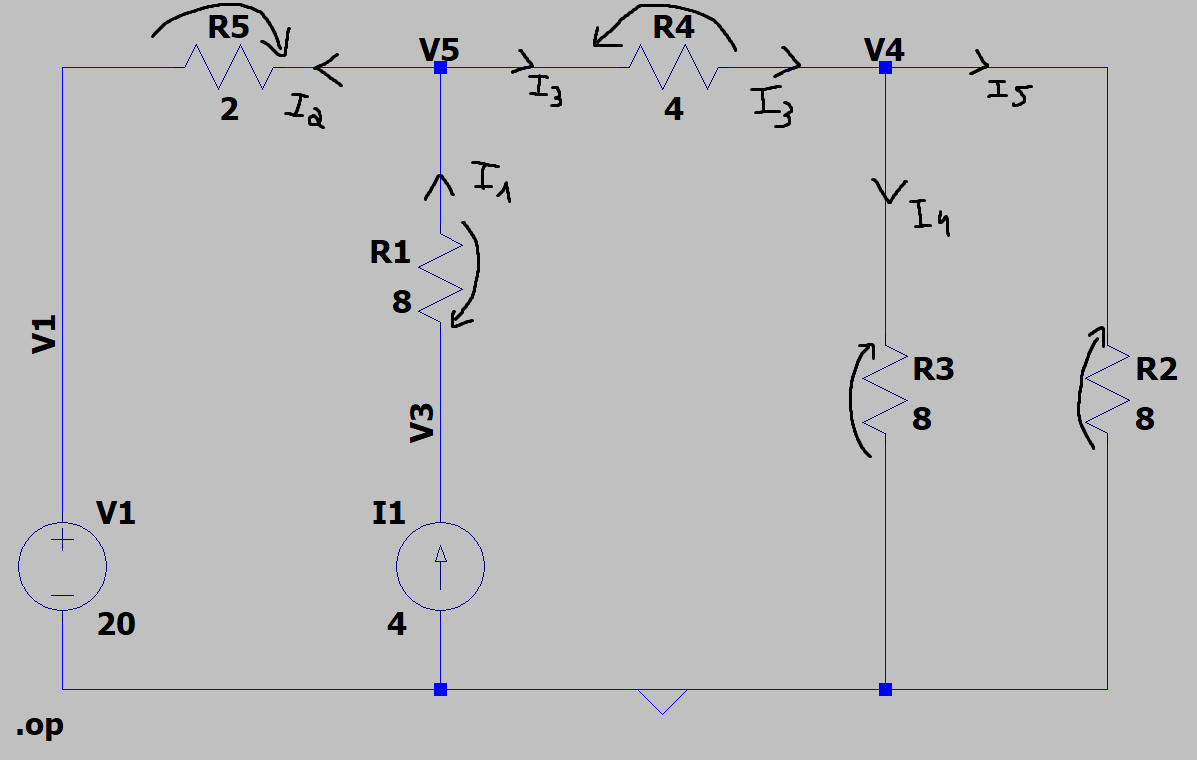
\includegraphics[scale=0.5]{Calculs.png}\\
        \large Mise en équation du circuit
    \end{center}
    
    On a les noeuds [2.1] et [2.2]
    \begin{align}
        I_1 = I_2 + I_3\\
        I_3 = I_4 + I_5\\
        I_1 = (V_3 - V_5) / R_1\\
        I_2 = (V_5 - V_1) / R_5\\
        I_3 = (V_5 - V_4) / R_4\\
        I_4 = V_4 / R_3\\
        I_5 = V_4 / R_2\\
    \end{align}
    
    On obtient V5 en terme de V4 en développant [2.2] et [2.5]
    \begin{align}
        I_3 = V_4 / R_3 + V_4 / R_2\\
        (V_5 - V_4) / R_4 = V_4 / R_3 + V_4 / R_2\\
        V_5 = 2V_4\\
    \end{align}
    
    On obtient la valeur de V4 et V5 en exprimant V5 en terme de V4 dans le noeud [2.1]
    \begin{align}
        I_3 = (2V_4 - V_4) / R_4 = V_4 / 4\\
        I_2 = (2V_4 - V_1) / R_5 = (2V_4 - 20) / 2\\
        I_1 = (2V_4 - 20) / 2 + V_4 / 4\\
        V_4 = 11,2\\
        V_5 = 2V_4 = 22,4\\
    \end{align}
    
    Grâce aux résultats déjà obtenu on calcul le reste du circuit
    \begin{align}
        I_1 = (V_3 - V_5) / R_1 = (V_3 - 22,4) / 8 = 4\\
        V_3 = 54,4\\
        I_2 = (2V_4 - 20) / 2 = 1,2\\
        I_3 = V_4/4 = 2,8\\
        I_4 = V_4 / R_3 = 11,2 / 8 = 1,4\\
        I_5 = V_4 / R_2 = 11,2 / 8 = 1,4
    \end{align}

\section{Conclusion}
    Les résultats obtenu sont en adéquation avec ceux obtenu lors de la simulation LTspice XVII.
    \begin{center}
        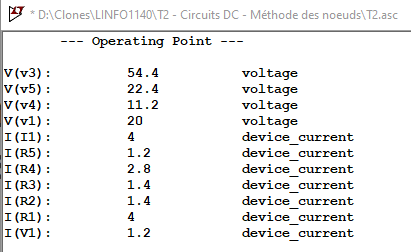
\includegraphics[scale=0.75]{Results.PNG}
    \end{center}
    \begin{itemize}
        \item La somme des courants entrant d'un noeud est bel et bien égale à la somme des courants sortant de ce même noeud.
    \end{itemize}
\end{document}
